\documentclass[aspectratio=169]{beamer}
\usetheme{Madrid}
\usecolortheme{whale}

\usepackage[utf8]{vietnam}
\usepackage{graphicx}
\usepackage{tikz}
\usetikzlibrary{arrows.meta,positioning}

\title{Lý thuyết đồ thị}
\subtitle{Cây và các thuật toán trên cây}
\author{Nhóm 7}
\date{\today}

\begin{document}

%------------------------------------------------
\begin{frame}
\titlepage
\end{frame}

%------------------------------------------------
\begin{frame}{Nội dung}
\tableofcontents
\end{frame}

%================================================
\section{Định nghĩa cây}

%------------------------------------------------
\begin{frame}{Cây là gì}

\begin{itemize}

    \item Cây là một loại đồ thị đặc biệt.
    \item Cây là đồ thị vô hướng, liên thông và không chứa chu trình.
    \item Cây có $n$ đỉnh sẽ có đúng $n-1$ cạnh.
    \item Hai đỉnh trong cây luôn có duy nhất một đường đi đơn.
    \item Cây không có chu trình nhưng nếu thêm vào một cạnh bất kỳ nối hai đỉnh không kề nhau, ta thu được duy nhất một chu trình.

\end{itemize}

\end{frame}

%------------------------------------------------
\begin{frame}{Ví dụ cây}
\begin{center}
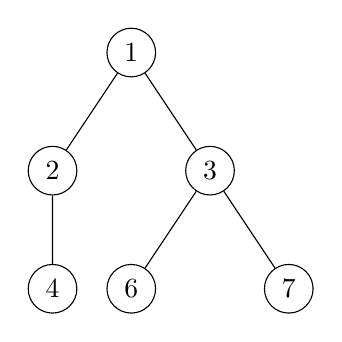
\begin{tikzpicture}[
    every node/.style={circle, draw, minimum size=0.6cm},
    level distance=1.5cm,
    sibling distance=2cm
]

\node {1}
    child {node {2}
        child {node {4}}
    }
    child {node {3}         
        child {node {6}
        }
        child {node {7}}
    };

\end{tikzpicture}
\end{center}
\end{frame}

%-----------------------------------------------
\begin{frame}{Các khái niệm quan trọng}

\begin{columns}

\column{0.55\textwidth}
\begin{itemize}
    \item \textbf{Bậc của đỉnh}: Số cạnh nối với đỉnh đó.
    \item \textbf{Đỉnh lá}: Đỉnh có bậc bằng 1.
    \item \textbf{Đỉnh gốc}: Đỉnh được chọn làm điểm xuất phát trong cây.
    \item \textbf{Cây con}: Cây con của một cây $T$ là một cây được tạo thành từ một đỉnh của $T$ và tất cả các đỉnh con của nó.
    \item \textbf{Đường đi}: Một dãy các đỉnh liên tiếp nhau trong cây, không lặp lại đỉnh nào.
    \item \textbf{Chiều cao của cây}: Số cạnh trên đường đi dài nhất từ gốc đến một đỉnh lá.
    \item \textbf{Độ sâu của đỉnh}: Số cạnh trên đường đi từ gốc đến đỉnh đó.
\end{itemize}

\column{0.45\textwidth}
\centering
\includegraphics[width=0.9\linewidth]{tree_concepts.jpg}

\end{columns}

\end{frame}
%------------------------------------------------

%================================================
\section{Ứng dụng của cây}

%------------------------------------------------
\begin{frame}{Ứng dụng}
\begin{itemize}
    \item Quản lí dữ liệu phân cấp (hệ thống tập tin, cơ sở dữ liệu).
    \item Thuật toán AI: cây quyết định (Decsion tree).
    \item Thuật toán tìm kiếm của Google,... (Trie).
    \item Sơ đồ tổ chức công ty.
    \item Hệ thống phân cấp nhà nước.
\end{itemize}
\end{frame}
%================================================
\section{Một số thuật toán trên cây}

%------------------------------------------------
\begin{frame}{Duyệt cây}

\begin{itemize}

\item Thường dùng thuật toán DFS để duyệt cây.
\item Dùng để tính chiều cao, độ sâu của câuy, đếm số đỉnh, tìm kiếm giá trị,...
\item Dùng trong DP trên cây.
\item Ý tưởng: Duyệt từ gốc, nếu các đỉnh kề không phải là cha của đỉnh hiện tại thì tiếp tục duyệt.

\end{itemize}

\begin{block}{Độ phức tạp}

\[
O(V+E)
\]

\end{block}

\end{frame}

%------------------------------------------------
\begin{frame}[fragile]{Code DFS trên cây}

\begin{verbatim}
void dfs(int u, int parent)
{
    for(int v : adj[u])
    {
        if(v != parent)
        dfs(v, u);
    }
}
\end{verbatim}

\end{frame}

%------------------------------------------------
\begin{frame}{Mô phỏng DFS trên cây}

\begin{center}

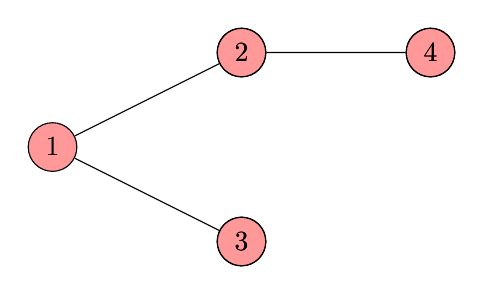
\begin{tikzpicture}[scale=1.2]

% Nodes
\node<1->[circle,draw,fill=red!40] (1) at (0,0) {1};

\node<2->[circle,draw,fill=red!40] (2) at (2,1) {2};
\node[circle,draw] (2a) at (2,1) {2};

\node<3->[circle,draw,fill=red!40] (4) at (4,1) {4};
\node[circle,draw] (4a) at (4,1) {4};

\node<4->[circle,draw,fill=red!40] (3) at (2,-1) {3};
\node[circle,draw] (3a) at (2,-1) {3};

% Edges (Tree)
\draw (1)--(2a);
\draw (2a)--(4a);
\draw (1)--(3a);

\end{tikzpicture}

\end{center}

\begin{itemize}
\item<1-> Bắt đầu từ đỉnh 1
\item<2-> Đi tới đỉnh 2
\item<3-> Đi tiếp tới đỉnh 4
\item<4-> Quay lui và thăm đỉnh 3
\end{itemize}

\end{frame}

%------------------------------------------------
\begin{frame}{Thuật toán Disjoint Set Union (DSU)}

\begin{itemize}
    \item \textbf{Bài toán:}
    \begin{itemize}
        \item Quản lý các tập hợp rời nhau
        \item Hỗ trợ gộp tập và kiểm tra cùng tập
    \end{itemize}

    \item \textbf{Ý tưởng cốt lõi:}
    \begin{itemize}
        \item Mỗi tập hợp được biểu diễn bởi một cây
        \item Mỗi phần tử lưu cha của nó
        \item Nút gốc là đại diện của tập
    \end{itemize}

    \item \textbf{Hai thao tác chính:}
    \begin{itemize}
        \item \textbf{Find(u)}: Tìm nút gốc chứa $u$
        \item \textbf{Union(u, v)}: Gộp hai tập bằng cách nối hai gốc
    \end{itemize}

    \item \textbf{Tối ưu quan trọng:}
    \begin{itemize}
        \item Path Compression: Nén đường đi khi Find
        \item Union by Size/Rank: Gộp cây nhỏ vào cây lớn
    \end{itemize}

    \item \textbf{Hiệu quả:} Độ phức tạp gần $O(1)$
\end{itemize}

\end{frame}

%------------------------------------------------
\begin{frame}[fragile]{Code DSU - khởi tạo}

\textbf{Ý tưởng:}
\begin{itemize}
    \item Mỗi đỉnh ban đầu là một tập riêng
    \item par[u] = -1 $\Rightarrow$ u là gốc của tập
    \item sz[u] = 1 $\Rightarrow$ kích thước tập bằng 1
\end{itemize}

\vspace{6pt}
\textbf{Cài đặt:}

%\scriptsize
\begin{verbatim}
ll par[N + 5], sz[N + 5], comps;

memset(par, -1, sizeof par);
fill(sz, sz + N + 2, 1);
\end{verbatim}

\end{frame}

%------------------------------------------------
\begin{frame}[fragile]{Code DSU — Find và Union}

\begin{columns}

\column{0.48\textwidth}
\textbf{Find(u)}
\begin{itemize}
    \item Tìm đại diện của tập chứa u
    \item Dùng Path Compression
\end{itemize}

\vspace{6pt}

\textbf{Union(u, v)}
\begin{itemize}
    \item Tìm hai gốc của u và v
    \item Nếu khác tập thì gộp lại
    \item Gộp cây nhỏ vào cây lớn
\end{itemize}

\column{0.52\textwidth}
\scriptsize
\begin{verbatim}
ll find(ll u)
{
    return par[u] == -1 ? u : par[u] = find(par[u]);
}

void union(ll u, ll v)
{
    u = find(u);
    v = find(v);
    if (u == v) return;

    if (sz[u] < sz[v]) swap(u, v);
    par[v] = u;
    sz[u] += sz[v];
}
\end{verbatim}

\end{columns}

\end{frame}

%------------------------------------------------
\begin{frame}{Mô phỏng DSU (Union-Find)}

\begin{center}
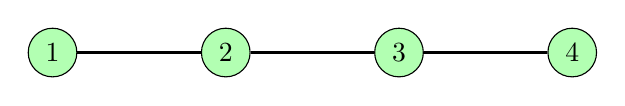
\begin{tikzpicture}[scale=1.1]

% ===== Step 1: Initial =====
\node<1->[circle,draw,fill=green!30] (1) at (0,0) {1};
\node<1->[circle,draw,fill=green!30] (2) at (2,0) {2};
\node<1->[circle,draw,fill=green!30] (3) at (4,0) {3};
\node<1->[circle,draw,fill=green!30] (4) at (6,0) {4};

% ===== Step 2: Union(1,2) =====
\draw<2->[thick] (1) -- (2);

% ===== Step 3: Union(3,4) =====
\draw<3->[thick] (3) -- (4);

% ===== Step 4: Union(2,3) =====
\draw<4->[thick] (2) -- (3);

\end{tikzpicture}
\end{center}

\begin{itemize}
\item<1-> Ban đầu: mỗi đỉnh là một tập riêng
\item<2-> Union(1,2): gộp tập chứa 1 và 2
\item<3-> Union(3,4): gộp tập chứa 3 và 4
\item<4-> Union(2,3): gộp hai tập lớn thành một
\end{itemize}

\end{frame}
%------------------------------------------------

\begin{frame}{Một số thuật toán phổ biến khác trên cây}
\begin{itemize}
    \item \textbf{LCA (Lowest Common Ancestor)}: Tìm tổ tiên chung thấp nhất của hai đỉnh.
    \item \textbf{Centroid Decomposition}: Phân tách cây thành các phần nhỏ hơn để giải quyết bài toán phức tạp.
    \item \textbf{Heavy-Light Decomposition}: Chia cây thành các chuỗi nặng và nhẹ để tối ưu truy vấn trên cây.
    \item \textbf{Dynamic Programming trên cây}: Sử dụng DP để giải quyết các bài toán tối ưu hóa trên cây.
    \item \textbf{Euler Tour Technique}: Biến đổi cây thành một mảng để giải quyết các bài toán truy vấn trên cây.
    \item \textbf{Centroid Tree}: Xây dựng cây centroid để giải quyết các bài toán liên quan đến khoảng cách trên cây.
\end{itemize}
\end{frame}
%================================================

\section{Kết luận}

%------------------------------------------------
\begin{frame}{Tổng kết}

\begin{itemize}
    \item Cây là đồ thị vô hướng liên thông, không có chu trình
    \item Với $n$ đỉnh luôn có đúng $n-1$ cạnh và duy nhất một đường đi giữa hai đỉnh
    \item Các thuật toán quan trọng: DFS/BFS, Tree DP, LCA
    \item Những bài toán về cây rất phổ biến trong lập trình thi đấu.
    \item Ứng dụng rộng rãi trong phân cấp dữ liệu và tối ưu mạng lưới
\end{itemize}

\end{frame}

%------------------------------------------------
\begin{frame}

\centering
\Huge
Cảm ơn các bạn đã lắng nghe!

\end{frame}

\end{document}